\begin{lstlisting}
习题2.3 第3、7、10题
习题2.4第6、8、11、14题
\end{lstlisting}
\begin{figure}[H]
\centering
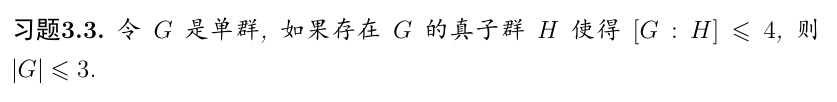
\includegraphics[width=\textwidth]{hw5-2025041223.png}
% \caption{}
\label{}
\end{figure}

\begin{proof}
There are 3 cases. $[G:H]=2,3$ or $4$.

If $[G:H]=2$ then $G=H\cup g_1H$. Consider the homomorphism
\[
\phi:G\to \mathrm{Aut}(H,g_1H)\cong \{ \pm1 \}\qquad g\mapsto l_{g}
\]
$l_{g}$ acts on $G$ by left multiplication,
\[
l_{g}:G\to G\qquad x\mapsto g\cdot x
\]
$\ker \phi =\{ 1 \}$, otherwise $\{ 1 \}\neq\ker \phi\lhd G$ then $G$ is not simple. Thus $G\cong\mathrm{Im}\phi\leq \{ \pm1 \}$, $\lvert G \rvert=2\Rightarrow G=\mathbb{Z}_{2}$.

If $[G:H]=3$ then $G=H\cup g_1H\cup g_2H$. Consider the homomorphism
\[
\phi:G\to \mathrm{Aut}(H,g_1H,g_2H)\cong S_3\qquad g\mapsto l_{g}
\]
$l_{g}$ acts on $G$ by left multiplication,
\[
l_{g}:G\to G\qquad x\mapsto g\cdot x
\]
$\ker \phi =\{ 1 \}$, otherwise $\{ 1 \}\neq\ker \phi\lhd G$ then $G$ is not simple. Thus $G\cong\mathrm{Im}\phi\leq S_3$. Since $S_3$ is not simple, $G\cong A_3\cong \mathbb{Z}_{3}$.

If $[G:H]=4$ then $G=H\cup g_1H\cup g_2H\cup g_3H$. Consider the homomorphism
\[
\phi:G\to \mathrm{Aut}(H,g_1H,g_2H,g_3H)\cong S_4\qquad g\mapsto l_{g}
\]
$l_{g}$ acts on $G$ by left multiplication,
\[
l_{g}:G\to G\qquad x\mapsto g\cdot x
\]
$\ker \phi =\{ 1 \}$, otherwise $\{ 1 \}\neq\ker \phi\lhd G$ then $G$ is not simple. Thus $G\cong\mathrm{Im}\phi\leq S_4$, $\lvert G \rvert|\lvert S_4 \rvert=24$. Also, $H\leq G$ implies that
\[
\lvert G \rvert =\lvert H \rvert \cdot[G:H]=4\lvert H \rvert
\]
$G$ is divisible by $4$. Thus $\lvert G \rvert=4,8,$ or $12$. If $\lvert G \rvert=4$ then $G\cong \mathbb{Z}_{4}$ or $\mathbb{Z}_{2}\times \mathbb{Z}_{2}$, not simple. If $\lvert G \rvert=8$ then $G\cong \mathbb{Z}_{2}\times\mathbb{Z}_{2}\times \mathbb{Z}_{2}$ or $\mathbb{Z}_{4}\times \mathbb{Z}_{2}$ or $\mathbb{Z}_{8}$, not simple. If $\lvert G \rvert=12$, it has a Sylow 3-subgroup, then $G$ is not simple.
\end{proof}

\begin{figure}[H]
\centering
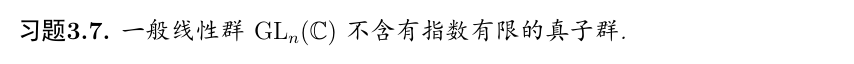
\includegraphics[width=\textwidth]{1-hw5-2025041223.png}
% \caption{}
\label{}
\end{figure}
\begin{proof}
Assume that $[\mathrm{GL}_n(\mathbb{C}):H]=m<\infty$, then $\mathrm{GL}_n(\mathbb{C})=H\cup g_1H\cup\dots \cup g_{m-1}H$. Consider
\[
\phi:\mathrm{GL}_n(\mathbb{C})\to \mathrm{Aut}(H,g_1H,\dots,g_{m-1}H)\cong S_m \qquad g\mapsto l_{g}
\]
$l_{g}$ acts on $\mathrm{GL}_n(\mathbb{C})$ by left multiplication,
\[
l_{g}:\mathrm{GL}_n(\mathbb{C})\to \mathrm{GL}_n(\mathbb{C})\qquad x\mapsto g\cdot x
\]
Then $\mathrm{GL}_n(\mathbb{C})/\ker \phi \cong \mathrm{Im}\phi \leq S_m$, thus $\lvert \mathrm{GL}_n(\mathbb{C})/\ker \phi \rvert\eqqcolon s|m!$. For any $A\in \mathrm{GL}_n(\mathbb{C})$, we have $A^{s}\in \ker \phi$. For any $B$ in $\mathrm{GL}_n(\mathbb{C})$, $B=A^{s}$ for some $A\in \mathrm{GL}_n(\mathbb{C})$, thus $B\in \ker \phi$, $\mathrm{GL}_n(\mathbb{C})=\ker \phi$. But $H=\ker \phi=G$ which is a contradiction.
\end{proof}
\begin{figure}[H]
\centering
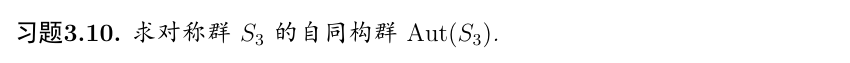
\includegraphics[width=\textwidth]{2-hw5-2025041223.png}
% \caption{}
\label{}
\end{figure}
\begin{proof}
\[
S_3=\{ 1,(1\ 2),(1\ 3),(2\ 3),(1\ 2\ 3),(1\ 3\ 2) \}
\]
\begin{figure}[H]
\centering
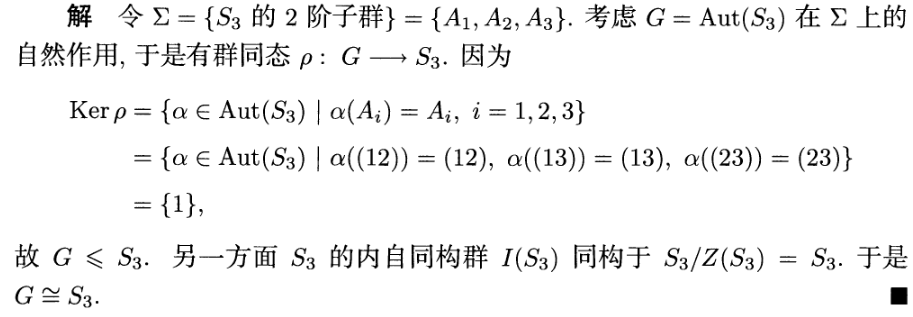
\includegraphics[width=\textwidth]{hw5-2025041301.png}
% \caption{}
\label{}
\end{figure}
\end{proof}

\begin{figure}[H]
\centering
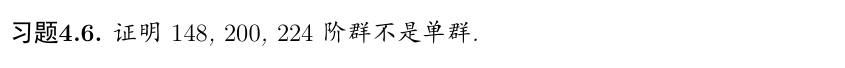
\includegraphics[width=\textwidth]{3-hw5-2025041223.png}
% \caption{}
\label{}
\end{figure}

\begin{proof}
(1) $\lvert G \rvert=148=2^2\times37$ then $n_{37}|4, n_{37}\equiv1(\mathrm{mod} \ 37)$ then $n_{37}=1$. By Sylow II theorem, the Sylow 37-subgroup is normal in $G$. Thus $G$ is not simple.

(2) $\lvert G \rvert=200=2^{3}\times5^2$, then $n_5|8,n_5\equiv1(\mathrm{mod}\ 5)$ then $n_5=1$. By Sylow II theorem, the Sylow 5-subgroup is normal in $G$. Thus $G$ is not simple.

(3) $\lvert G \rvert=224=2^{5}\times7$ then $n_7\in \{ 1,8 \}, n_2\in \{ 1,7 \}$. If $n_2=7$, denote the Sylow 2-subgroups by $P_1,P_2,\dots,P_7$. Then consider the homomorphism
\[
\phi:G\to \mathrm{Aut}\{ P_1,\dots,P_7 \}\cong S_7\qquad g\mapsto \mathrm{Ad}_{g}
\]
Assume that $\lvert G \rvert$ is simple, then $\ker \phi=\{ 1 \}$, $G\cong \mathrm{Im}\phi\leq S_7$, thus $\lvert G \rvert|\lvert S_7 \rvert=7!$. But $2^{5}\nmid 7!$, which is a contradiction. Therefore $G$ is not simple.
\end{proof}

\begin{figure}[H]
\centering
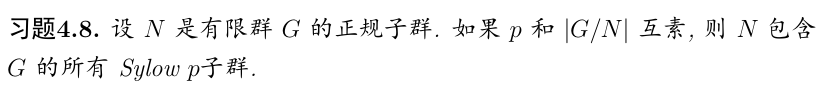
\includegraphics[width=\textwidth]{4-hw5-2025041223.png}
% \caption{}
\label{}
\end{figure}

\begin{proof}
$\lvert G \rvert=p^{r}m$, $p$ and $\lvert G/N  \rvert$ are relatively prime, then $N=p^{r}k$ for some $k|m$. By Sylow I theorem, $N$ contains a Sylow $p$ -subgroup $P$ with order $p^{r}$. $P$ is also a Sylow $p$ -subgroup of $G$. By Sylow II theorem, all Sylow $p$ -subgroups are conjugate to $P$, i.e. have the form $gPg^{-1}$ for some $g\in G$. NTS: $gPg^{-1}\subseteq N$. Since $N\lhd G$, $gPg^{-1}\subseteq N$ is equivalent to $P\subseteq g^{-1}Ng=N$, which is trivial. Hence $N$ contains all the Sylow $p$ -subgroups of $G$.
\end{proof}
\begin{figure}[H]
\centering
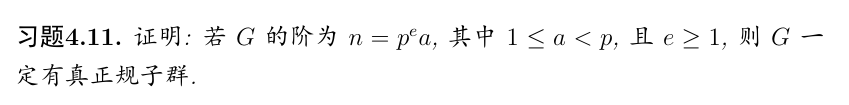
\includegraphics[width=\textwidth]{5-hw5-2025041223.png}
% \caption{}
\label{}
\end{figure}

\begin{proof}
$n_{p}|a, n_{p}\equiv1(\mathrm{mod}\ p)$. Since $1\leq a<p$, we have $n_{p}=1$. Thus the Sylow $p$ -subgroup is normal in $G$. When $a\neq1$, the Sylow $p$ -subgroup si proper normal subgroup of $G$. When $a=1$, if $e=1$ then $G$ has no proper normal subgroup. If $a=1,e\geq2$ then $\mathbb{Z}_{p^{e-1}}$ is proper normal subgroup of $G$.
\end{proof}
\begin{figure}[H]
\centering
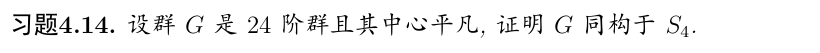
\includegraphics[width=\textwidth]{6-hw5-2025041223.png}
% \caption{}
\label{}
\end{figure}
$\lvert G \rvert=2^{3}\times3$. $n_2\in \{ 1,3 \}, n_3\in \{ 1,4 \}$.

If $n_3=1$, then by Sylow II theorem, the Sylow 3-subgroup $H$ is normal in $G$.

Unsolved...

\begin{note}
下面证明仅供参考而已,不是这样证明,但我太困了,下次再补. 下面的证明完全错误!
\begin{figure}[H]
\centering
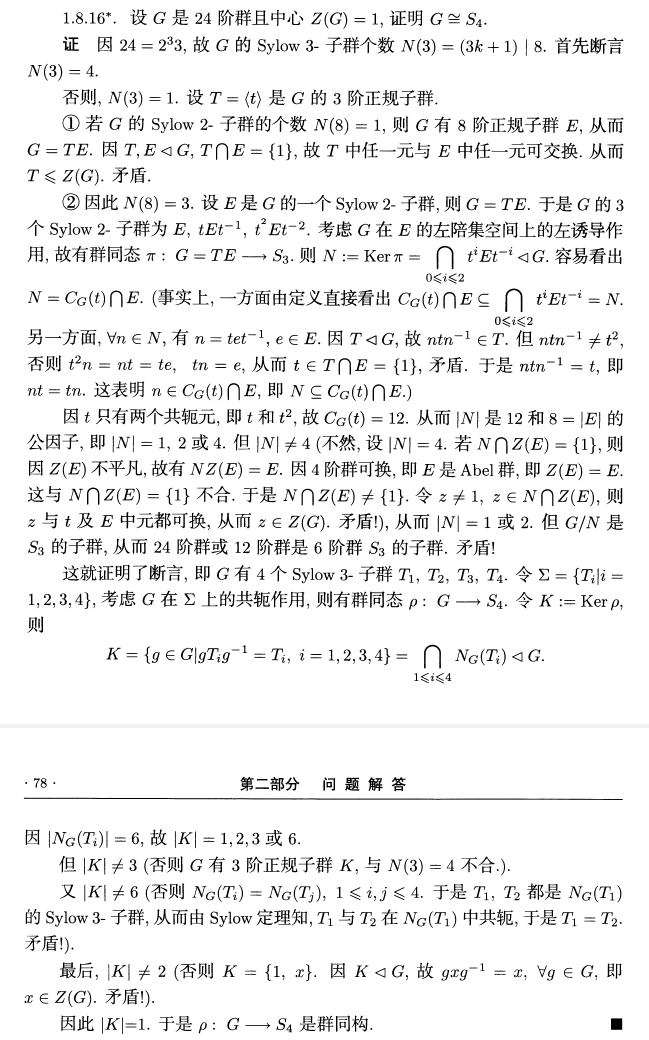
\includegraphics[width=\textwidth]{hw5-2025041400.png}
% \caption{}
\label{}
\end{figure}
\end{note}